\subsection{Quantum Gates and Circuits}
\label{subsec:gates}

Quantum gates are unitary operators ($U^\dagger U = I$). Key single-qubit gates include:
\begin{itemize}
    \item \textbf{Pauli-X}: Bit flip, $X = \begin{pmatrix} 0 & 1 \\ 1 & 0 \end{pmatrix}$.
    \item \textbf{Hadamard}: Creates superposition, $H = \frac{1}{\sqrt{2}}\begin{pmatrix} 1 & 1 \\ 1 & -1 \end{pmatrix}$.
    \item \textbf{Phase shift}: $R_\phi = \begin{pmatrix} 1 & 0 \\ 0 & e^{i\phi} \end{pmatrix}$.
\end{itemize}

The \textbf{CNOT gate} entangles qubits:
\[
\text{CNOT}|a\rangle|b\rangle = |a\rangle|a \oplus b\rangle.
\]

\begin{figure}[h]
\centering
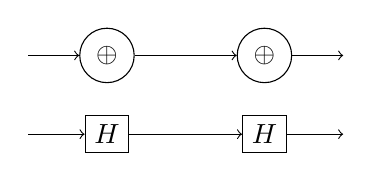
\begin{tikzpicture}
  \node[draw,circle] (cnot1) at (0,0) {$\oplus$};
  \node[draw,circle] (cnot2) at (2,0) {$\oplus$};
  \node[draw,rectangle] (h1) at (0,-1) {$H$};
  \node[draw,rectangle] (h2) at (2,-1) {$H$};
  \draw[->] (-1,0) -- (cnot1);
  \draw[->] (cnot1) -- (cnot2);
  \draw[->] (cnot2) -- (3,0);
  \draw[->] (-1,-1) -- (h1);
  \draw[->] (h1) -- (h2);
  \draw[->] (h2) -- (3,-1);
\end{tikzpicture}
\caption{Quantum circuit for the Deutsch-Jozsa algorithm.}
\label{fig:deutsch_circuit}
\end{figure}

Quantum circuits decompose algorithms into gate sequences. The \textbf{Quantum Fourier Transform} (QFT) is pivotal in Shor's algorithm \cite{shor1999polynomial}.